\PassOptionsToPackage{xetex}{xcolor}
\PassOptionsToPackage{xetex}{graphicx}
\documentclass[a4paper,landscape,headrule,footrule,xetex]{foils}

%%
%%%  Macros
%%%
\newcommand{\logo}{~}
\MyLogo{HG2052 (2020)}
%\newcommand{\Story}{\SHA{HOUN}{The Hound of the Baskervilles}}

\newcommand{\header}[3]{%
\title{\vspace*{-2ex} \Large HG2052
\\\large  Language, Technology and the Internet
\\[2ex] \Large  \emp{#2}}
\author{\blu{Francis Bond}   \\ 
\normalsize  \textbf{Division of Linguistics and Multilingual Studies}\\
\normalsize  \url{http://www3.ntu.edu.sg/home/fcbond/}\\
\normalsize  \texttt{bond@ieee.org}}
\MyLogo{HG2052 (2020)}
\date{#1}
\renewcommand{\logo}{#2}
 \hypersetup{
   pdfinfo={
     Author={Francis Bond},
     Title={#1: #2},
     Subject={HG2052: Language, Technology and the Internet},
     Keywords={Language, Technology, Internet},
     License={CC BY 4.0}
   }
 %  pdfcopyright={Copyright © Francis Bond. Creative Commons 4.0 Attribution License.}
 %  pdflicenseurl={http://creativecommons.org/licenses/by/4.0/}
 }
}


%%
%% Multilingual Stuff
%%
\usepackage[a4paper,landscape,margin=25mm]{geometry}

\usepackage{fontenc}
\usepackage{polyglossia}
\setmainlanguage{english}
\setmainfont{TeX Gyre Pagella}
%\setmainfont{Linux Libertine}
%\setmainfont{Charis SIL}
\newfontfamily{\ipafont}{Gentium}
\newcommand{\ipa}[1]{{\ipafont\selectfont #1}}
\usepackage{xeCJK}

\setCJKmainfont{Noto Sans CJK SC}
\setCJKsansfont{Noto Sans CJK SC}
%\setCJKttfont{Noto Sans CJK SC}
%\setCJKmainfont{WenQuanYi Micro Hei}
%\clearpage
%\setCJKmainfont{AR PL SungtiL GB}

\usepackage[xetex]{xcolor}
\usepackage[xetex]{graphicx}
\newcommand{\blu}[1]{\textcolor{blue}{#1}}
\newcommand{\grn}[1]{\textcolor{green}{#1}}
\newcommand{\hide}[1]{\textcolor{white}{#1}}
\newcommand{\emp}[1]{\textcolor{red}{#1}}
\newcommand{\txx}[1]{\textbf{\textcolor{blue}{#1}}}
\newcommand{\lex}[1]{\textbf{\mtcitestyle{#1}}}

\usepackage{pifont}
\renewcommand{\labelitemi}{\textcolor{violet}{\ding{227}}}
\renewcommand{\labelitemii}{\textcolor{purple}{\ding{226}}}

\newcommand{\subhead}[1]{\noindent\textbf{#1}\\[5mm]}

\newcommand{\Bad}{\emp{\raisebox{0.15ex}{\ensuremath{\mathbf{\otimes}}}}}
\newcommand{\bad}{*}

\newcommand{\com}[1]{\hfill \textnormal{(\emp{#1})}}%
\newcommand{\cxm}[1]{\hfill \textnormal{(\txx{#1})}}%
\newcommand{\cmm}[1]{\hfill \textnormal{(#1)}}%
\usepackage{amssymb}
\usepackage{relsize,xspace}
\newcommand{\into}{\ensuremath{\rightarrow}\xspace}
\newcommand{\ent}{\ensuremath{\Rightarrow}\xspace}
\newcommand{\nent}{\ensuremath{\not\Rightarrow}\xspace}
\newcommand{\tot}{\ensuremath{\leftrightarrow}\xspace}
\usepackage{url}
\usepackage[hidelinks]{hyperref}
\hypersetup{
     colorlinks,
     linkcolor={blue!50!black},
     citecolor={red!50!black},
     urlcolor={blue!80!black}
}
%\usepackage{hyperxmp}
\usepackage{url}
\newcommand{\lurl}[1]{\MyLogo{\url{#1}}}

\usepackage{mygb4e}
\let\eachwordone=\itshape
\newcommand{\lx}[1]{\textbf{\textit{#1}}}
\newcommand{\ix}{\ex\it}

\newcommand{\cen}[2]{\multicolumn{#1}{c}{#2}}
%\usepackage{times}
%\usepackage{nttfoilhead}
\newcommand{\myslide}[1]{%
\foilhead[-25mm]{\raisebox{12mm}[0mm]{\emp{#1}}}%
\leftheader{}%
\MyLogo{\logo}}

\newcommand{\mytask}[1]{%
\foilhead[-25mm]{\raisebox{12mm}[0mm]{\emp{#1}}}
\leftheader{🔍 Hi}%
\MyLogo{\logo}}

\newcommand{\myslider}[1]{\rotatefoilhead[-25mm]{\raisebox{12mm}[0mm]{\emp{#1}}}}
%\newcommand{\myslider}[1]{\rotatefoilhead{\raisebox{-8mm}{\emp{#1}}}}

\newcommand{\section}[1]{\myslide{}{\begin{center}\Huge \emp{#1}\end{center}}}

\usepackage{tcolorbox}
% \newcommand{\task}{\marginpar{\raisebox{-1ex}{\large
%       \tcbox[colframe=red,colback=white,arc=3pt]{\textbf{?}}}}}
% \newcommand{\task}{\marginpar{\raisebox{-1ex}{
%       \hspace{-0.5em}\tcbox[colframe=red,colback=white,arc=3pt]{%
%         \includegraphics[width=1.5em]{pics/detective}}}}}
\newcommand{\task}{\marginpar{\raisebox{-2ex}{
      \hspace{-0.5em}\reflectbox{\includegraphics[width=2em]{pics/detective}}}}}

\usepackage[lyons,j,e,k]{mtg2e}
\renewcommand{\mtcitestyle}[1]{\textcolor{teal}{\textsl{#1}}}
%\renewcommand{\mtcitestyle}[1]{\textsl{#1}}
\newcommand{\chn}{\mtciteform}
\newcommand{\cmn}{\mtciteform}
\newcommand{\iz}[1]{\textup{\texttt{\textcolor{blue}{\textbf{#1}}}}}
\newcommand{\con}[1]{\textsc{#1}}
\newcommand{\gm}{\textsc}
\newcommand{\cmp}[1]{{[\textsc{#1}]}}
\newcommand{\sr}[1]{\ensuremath{\langle}#1\ensuremath{\rangle}}
\usepackage[normalem]{ulem}
\newcommand{\ul}{\uline}
\newcommand{\uul}{\uuline}
\newcommand{\wl}{\uwave}
\newcommand{\vs}{\ensuremath{\Leftrightarrow}~}
%%%
%%% Bibliography
%%%
\usepackage{natbib}
%\usepackage{url}
\usepackage{bibentry}


%%% From Tim
\newcommand{\WMngram}[1][]{$n$-gram#1\xspace}
\newcommand{\infers}{$\rightarrow$\xspace}



\usepackage{rtrees,qtree}
\renewcommand{\lf}[1]{\br{#1}{}}
\usepackage{avm}
%\avmoptions{topleft,center}
\newcommand{\ft}[1]{\textsc{#1}}
\newcommand{\val}[1]{\textit{#1}}
\newcommand{\typ}[1]{\textit{#1}}
\avmfont{\sc}
%\avmvalfont{\sc}
\renewcommand{\avmtreefont}{\sc}
\avmsortfont{\it}


%%% From CSLI book
\newcommand{\mc}{\multicolumn}
\newcommand{\HD}{\textbf{H}\xspace}
\newcommand{\el}{\< \>}
\makeatother
\long\def\smalltree#1{\leavevmode{\def\\{\cr\noalign{\vskip12pt}}%
\def\mc##1##2{\multispan{##1}{\hfil##2\hfil}}%
\tabskip=1em%
\hbox{\vtop{\halign{&\hfil##\hfil\cr
#1\crcr}}}}}
\makeatletter

\newcommand{\sh}[1]{\href{https://www.arthur-conan-doyle.com/index.php?title=#1}{#1}}
\newcommand{\SHA}[2]{\href{https://www.arthur-conan-doyle.com/index.php?title=#1}{\textit{#2}}}


\header{Lecture 12}{Review and Conclusions}



\begin{document}

\bibliographystyle{apalike}
\nobibliography{abb,mtg,nlp,ling}

\maketitle




\section{Introduction}

\myslide{What have we learned?}

\begin{itemize}
\item How technology affects our use of language
% (from the effects of encoding to the rise of chatspeak), and also
 \item How language is used on the internet
   \begin{itemize}
   \item Some interesting things we can now do, that we couldn't before 
   \end{itemize}
 \item Collaboration on the Web
 \item The web as a source of linguistic data: Direct Query and Sample
 \item The Semantic Web: meaning for non-humans
 \item Citation and reputation
%   Students will gain understanding of the 
% problems of representing, transmitting and transforming language
% electronically.  Specific topics will include automatic parsing and
% generation of language, text mining (extracting knowledge from text)
% and machine translation.
\end{itemize}

\myslide{Reflection}
\begin{itemize}
\item What was the most surprising thing in this class?
\item What do you think is most likely wrong?
\item What do you think is the coolest result?
\item What do you think you’re most likely to
remember?
\item How do you think this course will influence you as a linguist?
\item What (if anything) did you hope to learn that you didn't?
\end{itemize}



\myslide{Goals}
\begin{itemize}
\item Gain an understanding of how technology affects language use
\item Develop familiarity with markup and meta information in texts
\item Get a feel for what research is all about, especially relating to
  web mining and online frequency counting
\end{itemize}
\subhead{Upon successful completion, students will:}
\begin{itemize}
\item have an understanding of how technology shapes language use
\item be able to test linguistic hypotheses against web data.
\item know how to edit Wikipedia
\end{itemize}






\myslide{Themes}
\begin{itemize}
\item Language and Technology
  \begin{itemize}
  \item Writing and Speech Technology
  \end{itemize}
\item Language and the Internet
  \begin{itemize}
  \item Email; Chat; Virtual Worlds; WWW; \ul{IM; Blogs}; \uul{Facebook; Wikis; Twitter}
  \end{itemize}
\item The Web as Corpus
\item The Web beyond Language
  \begin{itemize}
  \item Semantic Web and Networks
  \end{itemize}
\end{itemize}

% \myslide{Improvised Teaching}

% \begin{itemize}
% \item What do you want to know (related to Language, Technology and
%   the Internet)?
%   \begin{itemize}
%   \item You have 10 minutes to think of questions
%   \item I will pick 5 and try to answer them
% \\ You can try to answer them as well, \ldots 
%   \end{itemize}
% \end{itemize}


\section{Revision}


\myslide{Language and Technology}

\begin{itemize}
\item The two things that separate humans from animals \citep[\S1.1]{Sproat:2010}
  \begin{itemize}
  \item Language
    \begin{itemize}
    \item large vocabulary (10,000+)
    \item complicated syntax (no upper length; recursion; embedding)
    \end{itemize}

  \item Technology
    \begin{itemize}
    \item Widespread tool use
    \item Widespread tool manufacture
    \end{itemize}
  \end{itemize}
\item Speech --- the start of language 
\item Writing --- the first great intersection
\end{itemize}


\myslide{Language and the Internet}

\begin{itemize}
\item New forms of communication
  \begin{itemize}
  \item Neither speech nor text
  \item Massively interactive
  \end{itemize}
\item Extremely rapid change
\item A first hand narrative (I was online before the internet :-)
  \begin{itemize}
  \item but I am probably behind you all now
  \end{itemize}
\end{itemize}


\myslide{New forms}
\begin{itemize} 
\item Email (from PC, phone, other)
\item Chat; Usenet
\item Virtual Worlds
\item WWW
\item Blogs (overlap)
\item Facebook, LinkedIn
\item Wikis
\item Twitter
\end{itemize}




\section{Representing Language}

\begin{itemize}
\item Writing Systems
\item Encodings
\item Speech
\item Bandwidth
\end{itemize}


\myslide{What is represented?}
%%% FIXME
\begin{itemize}
\item \ul{\blu{Phonemes}}:  \ipa{/maɪ dɒg laɪks ˈɒrɪnʤɪz/}  \com{45}
  \begin{itemize}
  \item Not a  simple correspondence between a writing system
    and the sounds
  \item Some logographs (\textit{3}, \textit{@}, \textit{\$})
  \item Even when a new alphabet is designed, pronunciation changes.
  \end{itemize}
\item Syllables:  \ipa{maɪ dɒg laɪks (ˈɒr)(ɪn)(ʤɪz)}  \com{10,000+}
\item Morphemes: my/me+'s dog like+s orange+s \com{100,000+}
\item Words: \eng{my dog likes oranges} \com{200,000+}
\item Concepts: \iz{speaker poss dog$_{canine}$:SG fond orange$_{fruit}$:PL}  \com{400,000++}
\end{itemize}


\myslide{Three Major Writing Systems}
\begin{itemize}
\item Alphabetic (Latin)
  \begin{itemize}
  \item  one symbol for consonant or vowel
  \item Typically 20-30 base symbols (1 byte)
  \end{itemize}
\item Syllabic (Hiragana)
  \begin{itemize}
  \item  one symbol for each syllable (consonant+vowel)
  \item Typically 50-100 base symbols (1-2 bytes)
  \end{itemize}
\item Logographic (Hanzi)
  \begin{itemize}
  \item pictographs, ideographs, sounds-meaning combinations
  \item Typically 10,0000+ symbols (2-3 bytes)
  \end{itemize}


\end{itemize}
\myslide{Computational Encoding}

\begin{itemize}
\item Need to map characters to bits
\item More characters require more space
  \begin{itemize}
  \item English: ASCII (7 bits); Western Europe: ISO-8859-1 (8 bits); 
    \\ Japanese: EUC (16 bits); Everything: UTF-8 (8-32 bits)
  \end{itemize}
\item Moving towards unicode for everything
\item If you get the encoding wrong, it is gibberish
  \begin{itemize}
  \item Web pages should state their encoding
  \item Sometimes they are wrong
  \item \blu{Encoding Detection}  usually involves statistical analysis of byte patterns
    \begin{itemize}
    \item But an encoding can be shared by many languages
    \end{itemize}
  \end{itemize}
\end{itemize}




\section{Speech and Language Technology}

\begin{itemize}
\item The need for speech representation
\item Storing sound
\item Transforming Speech
  \begin{itemize}
  \item \blu{Automatic Speech Recognition (ASR)}: sounds to text
  \item \blu{Text-to-Speech Synthesis (TTS)}: texts to sounds
  \end{itemize}
\item Speech technology --- the Telephone!
\end{itemize}


\myslide{How good are the systems?}

  \begin{tabular}{lrrr}
    Task & Vocab & WER (\%) & WER  (\%) adapted \\ \hline
    Digits & 11 & 0.4 & 0.2 \\
    Dialogue (travel) & 21,000 & 10.9 & --- \\
    Dictation (WSJ) & 5,000 & 3.9 & 3.0 \\
    Dictation (WSJ) & 20,000 & 10.0 & 8.6 \\
    Dialogue (noisy, army) & 3,000 & 42.2 & 31.0 \\
    Phone Conversations & 4,000 & 41.9 & 31.0 \\
  \end{tabular}

Results of various DARPA competitions (from Richard Sproat's slides)

\myslide{Why is it so difficult?}
\begin{itemize}
\item Pronunciation depends on context
  \begin{itemize}
  \item The same word will be pronounced differently in different sentences
  \end{itemize}
\item Speaker variability
  \begin{itemize}
  \item Gender
  \item Dialect/Foreign Accent
  \item Individual Differences: Physical differences; Language differences (idiolect)‏
  \end{itemize}
\item Many, many rare events
  \begin{itemize}
  \item 300 out of 2000 diphones in the core set for the AT\&T NextGen system occur only once in a 2-hour speech database
  \end{itemize}
\end{itemize}


\myslide{Two steps in a TTS system}

\begin{enumerate}
\item Linguistic Analysis
  \begin{itemize}
  \item Sentence Segmentation
  \item Abbreviations: \eng{Dr Smith lives on Nanyang Dr. He is \ldots}
  \item Word Segmentation: 
    \begin{itemize}
    \item 森山 前 日銀 総裁 \jpn{Moriyama zen Nichigin Sousai}
    \item[\Bad]  森山 前日 銀 総裁 \jpn{Moriyama zennichi gin Sousai}
      \end{itemize}
    \end{itemize}
\item Speech Synthesis
  \begin{itemize}
  \item Find the pronunciation
  \item Generate sounds
  \item Add intonation
  \end{itemize}
\end{enumerate}

\myslide{Speech Synthesis}
  \begin{itemize}
  \item \blu{Articulatory Synthesis:} Attempt to model human articulation.
  \item \blu{Formant Synthesis:} Bypass modeling of human articulation, and model acoustics directly.
  \item \blu{Concatenative Synthesis:} Synthesize from stored units of actual speech
  \end{itemize}
  
\myslide{Prosody of Emotion}

\begin{itemize}
\item Excitement: Fast, very high pitch, loud
\item Hot anger: Fast, high pitch, strong, falling accent, loud
\item Fear: Jitter
\item Sarcasm: Prolonged accent, late peak
\item Sad: Slow, low pitch
\end{itemize}

\begin{quote}
  The main determinant of ``naturalness'' in speech synthesis is not
  ``voice quality'', but natural-sounding prosody (intonation and
  duration) 
  \begin{flushright}
    Richard Sproat
  \end{flushright}
\end{quote}




\myslide{Speed is different for different modalities}
% http://en.wikipedia.org/wiki/Words_per_minute
Speed in words per minute (one word is 6 characters)
\\ (English, computer science students, various studies)

\begin{tabular}{lrl}
  Reading            & 300 & 200 (proof reading)\\
  Writing              & 31 & 21 (composing) \\ 
  Speaking             & 150 & \\
  Hearing              & 150 & 210 (speeded up)  \\
  Typing               & 33  & 19 (composing) 
\end{tabular}
\begin{itemize}
\item Reading $>>$ Speaking/Hearing $>>$ Typing
  \begin{itemize}
  \item[$\Rightarrow$] Speech for input
  \item[$\Rightarrow$] Text for output
  \end{itemize}
\end{itemize}



\myslide{The Telephone}

\begin{tabular}{ll}
  \textbf{Speech like} & \textbf{Text like} \\ \hline
  \blu{time bound} & space bound \\
  \blu{spontaneous} & contrived \\
  face-to-face & \blu{visually decontextualized} \\
  \blu{loosely structured} & elaborately structured \\
  \blu{socially interactive} & factually communicative \\  
  \blu{immediately revisable} & repeatedly revisable \\
  \blu{prosodically rich} & graphically rich \\
\end{tabular}


\section{New Modalities}

\myslide{Email; Usenet; Chat and Blogs}

\begin{itemize}
\item All share some characteristics of speech and text
\item Usage norms not fixed
\item Communication methods may disappear before the norms are fixed
\\ Usenet, Bulletin Boards, Gopher, Archie, \ldots
\item Large scale discourse studies still to be done
\item Some genuinely new things
  \begin{itemize}
  \item time-lagged, multi-person conversation
  \item raw un-edited text
  \item extreme multi-authorship
  \end{itemize}
\end{itemize}

\myslide{Email}


\begin{tabular}{ll}
  \textbf{Speech like} & \textbf{Text like} \\ \hline
  \blu{time bound}* &  \blu{space bound} (deletable) \\
  \blu{spontaneous}* & \blu{contrived}* \\
  face-to-face & \blu{visually decontextualized} \\
  \blu{loosely structured}* & \blu{elaborately structured}* \\
  \blu{socially interactive}* & \blu{factually communicative} \\  
  immediately revisable & \blu{repeatedly revisable}* \\
  prosodically rich & graphically rich * \\
\end{tabular}


\myslide{Usenet (asynchronous)}


\begin{tabular}{ll}
  \textbf{Speech like} & \textbf{Text like} \\ \hline
  \blu{time bound}* &  \blu{space bound} \\
  \blu{spontaneous}* & \blu{contrived}* \\
  face-to-face & \blu{visually decontextualized} \\
  \blu{loosely structured}* & elaborately structured \\
  \blu{socially interactive}* & \blu{factually communicative} \\  
  immediately revisable & repeatedly revisable \\
  prosodically rich & graphically rich  \\
\end{tabular}



\myslide{Chat (synchronous)}


\begin{tabular}{ll}
  \textbf{Speech like} & \textbf{Text like} \\ \hline
  \blu{time bound}* &  \blu{space bound} \\
  \blu{spontaneous}* & contrived \\
  face-to-face & \blu{visually decontextualized} \\
  \blu{loosely structured}* & elaborately structured \\
  \blu{socially interactive}* & \blu{factually communicative} \\  
  immediately revisable & repeatedly revisable \\
  prosodically rich & graphically rich  \\
\end{tabular}


\myslide{Blogs}


\begin{tabular}{ll}
  \textbf{Speech like} & \textbf{Text like} \\ \hline
  time bound &  \blu{space bound} \\
  \blu{spontaneous}* & \blu{contrived}* \\
  face-to-face & \blu{visually decontextualized} \\
  \blu{loosely structured}* & \blu{elaborately structured}* \\
  \blu{socially interactive}$^{comments}$ & \blu{factually communicative} \\  
  immediately revisable & \blu{repeatedly revisable}* \\
  prosodically rich & graphically rich * \\
\end{tabular}

\myslide{Netspeak}
\begin{itemize}
\item Inspired by shared background
  \begin{itemize}
  \item \url{<rant>}I can't stand this\url{</rant>}
  \item I hate\url{^H^H^H^H}love that idea \hfill (\url{^H} is backspace on a vt100)
  \item lusers (users as seen by Systems Administrators)
  \item suits
  \end{itemize}
\item Need to be in-group: 
  \begin{description}
  \item[cow orker] Coworker
  \item[clue] ``You couldn't get a clue during the clue mating season in a field full of horny clues if you smeared your body with clue musk and did the clue mating dance.''
\\ Edward Flaherty (\url{talk.bizaare})
  \end{description}
\newpage
\item Gricean Principals
  \begin{itemize}
  \item Posting (top/middle/bottom, quoting and trimming)
  \end{itemize}

\item Inspired by medium limitations
  \begin{itemize}
  \item \url{GREAT; *great*;  g r e a t}
  \item \url{:-)}\ \ \ \ \ \url{(^_^)} \ \ \ \  \url{(;o;)}\ \ \ \ $\ddot\smile$
  \item \url{brb}, \url{RTFM}, \url{IMHO}
  \item lower case
  \item lack of punctuation (hard on phone keyboards)
  \end{itemize}

\end{itemize}

\section{Collaboration and Wikis}

\MyLogo{}
\begin{itemize}
\item Version Control Systems
\item Wikipedia
\item Licensing and Ownership 
\end{itemize}

\myslide{Version Control Systems}

\begin{itemize}
\item Versioning file systems
  \begin{itemize}
  \item  every time a file is opened, a new copy is stored
  \end{itemize}
\item CVS, Subversion, Git
  \begin{itemize}
  \item changes to a collection of files are tracked
  \item simultaneous changes are merged
  \end{itemize}
\item Revision Tracking
  \begin{itemize}
  \item Revisions are stored within a file
  \end{itemize}
\item Authorship in shared writing; Explicit responsibility for changes
\end{itemize}

\myslide{Wikipedia}
\begin{itemize}
\item  The core aim of the Wikimedia Foundation, is to get a free
  encyclopedia to every single person on the planet. (Jimmy Wales)
\item Wikipedia makes it easy to share your knowledge
 \\ people like to do this
\item Most edits are done by insiders
\item Most content is added by outsiders
\item Content comparable to Britannica
\end{itemize}

\myslide{The five pillars of Wikipedia}
\MyLogo{\url{Wikipedia:Five pillars}}
\begin{enumerate}
\item Wikipedia is an online encyclopedia
\item Wikipedia has a neutral point of view
  \begin{itemize}
  \item Content policies:  NPOV, Verifiability, and No original research
  \end{itemize}
\item Wikipedia is free content
\item Wikipedians should interact in a respectful and civil manner
\item Wikipedia does not have firm rules
\end{enumerate}

\myslide{Licenses and Ownership}

\begin{itemize}
\item Copyright
\item Copyleft
\item Creative Commons
\end{itemize}

\myslide{What is a good article?}
\MyLogo{\url{Wikipedia:Good_article_criteria}}

\begin{enumerate}
\item Well-written
\item Factually accurate and verifiable
\item Broad in its coverage
\item Neutral
\item Stable
\item Illustrated, if possible, by images
\end{enumerate}


\section{The World Wide Web and HTML}

\myslide{The InterWeb}

\begin{itemize}
\item The Internet
   \\ more than just the web (email, VoIP, FTP, Streaming, Messaging~
\item The structure of Markup: Visual vs Logical
  \\ WSISWYG; WYSIAYG; WYSIWIM
\item The structure of the Web --- hypertext
\\ pages linked to pages
\item The future of the Web
\item Linguistic features of the web
 \\ un-edited; large volume; editable; multi-media
\end{itemize}

\myslide{Map of online communities}
\MyLogo{\url{http://xkcd.com/802/}}

\begin{center}
  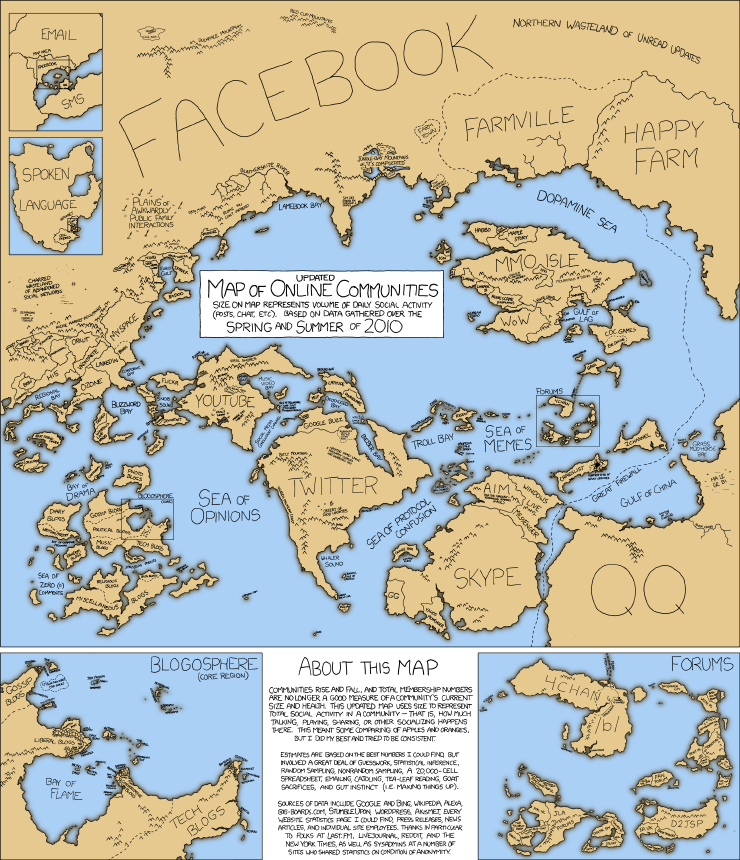
\includegraphics[height=\textheight]{../pics/online_communities_2}
\end{center}


\myslide{The Deep Web (the Invisible Web)}
\begin{description}
\item [Dynamic content] dynamic pages which are returned in response to a submitted query or accessed only through a form
\item [Unlinked content] pages which are not linked to by other pages (but clicking links them)
\item [Private Web] sites that require registration and login \com{Edventure}
\item [Contextual Web] pages with content varying for different access contexts (e.g., ranges of client IP addresses or previous navigation sequence).
\item [Limited access content] sites that limit access to their pages
  in a technical way (e.g., using the Robots Exclusion Standard)
\item [Scripted content] pages that are only accessible through links produced by JavaScript as well as content dynamically downloaded from Web servers via Flash or Ajax solutions.
\item [Non-HTML/text content] textual content encoded in multimedia (image or video) files or specific file formats not handled by search engines.
\end{description}

These pages all include data that search engines cannot find!

\myslide{Visual Markup vs Logical Markup}

\begin{itemize}
\item Visual Markup (Presentational)
  \begin{itemize}
  \item What you see is what you get (WYSIWYG)
  \item Equivalent of printers' markup
  \item Shows what things look like
  \end{itemize}
\item Logical Markup (Structural)
  \begin{itemize}
  \item Show the structure and meaning
  \item Can be mapped to visual markup
  \item Less flexible than visual markup
  \item More adaptable (and reusable)
  \end{itemize}
\end{itemize}




\section{The Web as Corpus}
\myslide{Two Approaches to using the Web as a Corpus}
\begin{itemize}
\item \blu{Direct Query}: Search Engine as Query tool and WWW as corpus?
\\  (Objection: Results are not reliable)
\begin{itemize}
\item Population and exact hit counts are unknown → no statistics
possible.
\item Indexing does not allow to draw conclusions on the data.
\item[\Bad] Google is missing functionalities that linguists /
lexicographers would like to have.
\end{itemize}
\item \blu{Web Sample}: Use search engine to download data from the
net and build a corpus from it.
\begin{itemize}
\item known size and exact hit counts → statistics possible.
\item people can draw conclusions over the included text types.
\item (limited) control over the content.
\item[\Bad] sparser data
\end{itemize}
\end{itemize}

\myslide{Direct Query}
\begin{itemize}
\item Accessible through search engines (Google API, Yahoo API, Scripts)

\item Document counts are shown to correlate directly with ``real''
  frequencies (Keller 2003), so search engines can help - but...
  \begin{itemize}
  \item lots of repetitions of the same text (not representative)
  \item very limited query precision (no upper/lower case, no punctuation...)
  \item only estimated counts, often hard to reproduce exactly
  \item different queries give wildly different numbers
  \end{itemize}
\end{itemize}

\myslide{Web Count Units}
\MyLogo{http://itre.cis.upenn.edu/~myl/languagelog/archives/000953.html}

\begin{itemize}\addtolength{\itemsep}{-1ex}
\item \blu{ghit} or ``google hit'' is the most common unit used to
  count web snippets (in the early 2000s)
  \begin{itemize}
  \item it is document frequency not term frequency
  \end{itemize}
\item \blu{whit} or ``web hit'' is the more general term
\item Normally you compare two phenomena to get a unitless ratio
  \\(e.g. \eng{different from} vs \eng{different than})
  \\ 251,000,000 ghits vs 71,500,000 or \emp{3.5:1} (accessed 2012-04-04)
%(/ 251 71.5) 3.5104895104895104
\item \blu{GPB}, for ``Ghits per billion documents'' is good if want a
  more stable number (suggested by Mark Liberman)
\\ but Google no longer releases the index size 
\item So always say when you counted, and try to use ratios
\end{itemize}

\myslide{Web Sample}
\MyLogo{}
\begin{itemize}
\item Extracting and filtering web documents to create linguistically
  annotated corpora (Kilgarriff 2006)
  \begin{itemize}
  \item gather documents for different topics (balance!)
  \item exclude documents which cannot be preprocessed with available
    tools (here taggers and lemmatizers)
  \item exclude documents which seem irrelevant for a corpus (too short or
    too long, word lists,...)
  \item do this for several languages and make the corpora available
  \end{itemize}
\end{itemize}


\myslide{Building Internet Corpora: Outline}
\MyLogo{\url{http://corpus.leeds.ac.uk/internet.html}}

\begin{enumerate}
\item Select Seed Words (500)
\item Combine to form multiple queries (6,000)
\item Query a search engine and retrieve the URLs (50,000)
\item Download the files from the URLS (100,000,000 words)
\item Postprocess the data (encoding; cleanup; tagging and parsing)
\end{enumerate}

Sharoff, S (2006) Creating general-purpose corpora using automated search engine queries. In M. Baroni, S. Bernardini (eds.) WaCky! Working papers on the Web as Corpus, Bologna, 2006.

\myslide{Internet Corpora Summary}
\MyLogo{}
 
\begin{itemize}
\item The web can be used as a corpus
  \begin{itemize}
  \item Direct access
    \begin{itemize}
    \item Fast and convenient
    \item Huge amounts of data
    \item[\Bad] unreliable counts 
    \end{itemize}
  \item Web sample
    \begin{itemize}
    \item Control over the sample
    \item Some setup costs (semi-automated)
    \item[\Bad] Less data 
    \end{itemize}
  \end{itemize}
\item Richer data than a compiled corpus
\item[\Bad] Less balanced, less markup
\end{itemize}





\section{Text and Meta-text}
\MyLogo{and Zombies}
\begin{itemize}
\item Explicit Meta-data
  \begin{itemize}
  \item Keywords and Categories
  \item Rankings
  \item Structural Markup
  \end{itemize}
\item Implicit Meta-data
  \begin{itemize}
  \item Links and Citations
  \item Tags
  \item Tables
  \item File Names
  \item Translations
  \end{itemize}
\end{itemize}

\myslide{Explicit Metadata}
\MyLogo{}
\begin{itemize}
\item You can get information from metadata within documents
  \begin{itemize}
  \item When they are accurate they are very good
  \item They are often deceitful
  \end{itemize}
\item HTML, PDF, Word, \ldots Metadata
\item Keywords and Tags
\item Rankings
\item Links and Citations
\item Structural Markup
\end{itemize}

\myslide{Implicit Metadata}
\begin{itemize}
\item You can get clues from metadata within documents
  \begin{itemize}
  \item as they are non-intended, they tend to be noisy
  \item but they are rarely deceitful
  \end{itemize}
\item HTML tags as constituent boundaries
\item Tables as Semantic Relations
\item File Names (content type and language)
\item Translations ---  Bracketed Glosses;  Cross-lingual Disambiguation
\item Query Data
\item Wikipedia Redirections and Cross-wiki Links
\end{itemize}

\section{Language Identification and Normalization}

\myslide{Language Identification}

\begin{itemize}
\item Need to identify the encoding and language of a page in order to
  process it (meta-data may be unreliable)
  \begin{itemize}
  \item Linguistically-grounded methods
    \begin{itemize}
    \item Diacritics
    \item Character $n$-grams
    \item Stop words
    \end{itemize}
  \item Similarity-based categorisation and classification
    \begin{itemize}
    \item  Character $n$-gram rankings
    \end{itemize}
  \item Machine Learning based methods
\item Context (under \url{.jp} or \url{.ko}?)
  \end{itemize}
\item Hard to do for short test snippets, similar languages, mixed text

\end{itemize}

\myslide{Normalization}

\begin{itemize}
\item Extracting text from various documents
\item Segmenting continuous text
\item Number Normalization:  
  \eng{\$700K}, \eng{\$700,000}, \eng{0.7 million dollars},  \ldots
\item Date Normalization:   \eng{2000AD, 1421AH,  Heisei 12, \ldots} 
\item Stripping stop words (\lex{the}, \lex{a}, \lex{of}, \ldots)
\item Lemmatization:  \eng{produces}   \infers \lex{produce}
\item Stemming:  \eng{producer}   \infers \eng{produc}; \eng{produces}   \infers \eng{produc}
\item Decompounding: \eng{zonnecel}  \infers \eng{zon cel}
\end{itemize}



\section{The Semantic Web}
\myslide{Goals of the Semantic Web}
\begin{itemize} 
\item Web of data
  \begin{itemize}
  \item provides common data representation framework
  \item makes possible integrating multiple sources
  \item so you can draw new conclusions
  \end{itemize}
\item  Increase the utility of information by connecting it to definitions and context
\item  More efficient information access and analysis
\end{itemize}

E.G. not just "color" but a concept denoted by a Web identifier: 
\\ \url{<http://pantone.tm.example.com/2002/std6#color>}

\myslide{Semantic Web Architecture}

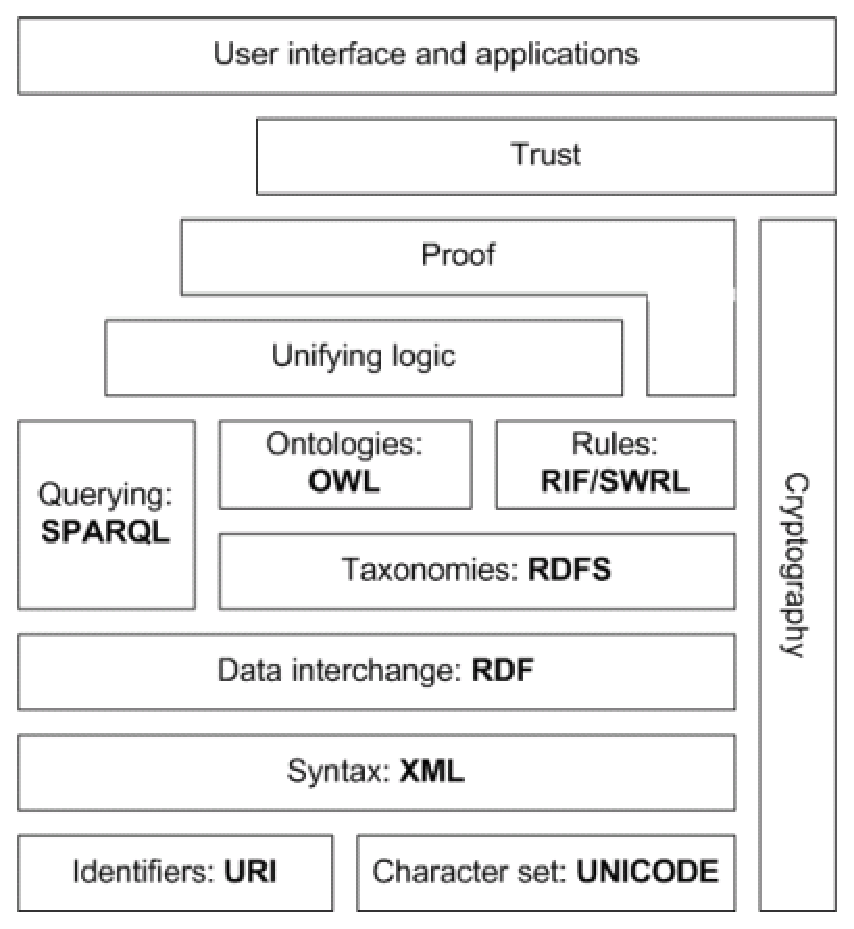
\includegraphics[height=\textheight]{../pics/semantic-web-layers.eps}

\myslide{XML: eXtensible Markup Language}

\begin{itemize}
\item XML is a set of rules for encoding documents electronically.
  \begin{itemize}
  \item is a markup language much like HTML
  \item was designed to \blu{carry data, not to display data}
  \item tags are not predefined. You must define your own tags
  \item is designed to be \blu{self-descriptive}
  \item XML is a W3C Recommendation
  \end{itemize}
  \item Can be validated for syntactic well-formedness
\end{itemize}


\myslide{Semantic Web Architecture (details)}
\begin{itemize}
\item Identify things with  \blu{Uniform Resource Identifiers}
  \begin{itemize}
  \item \blu{Universal Resource Name}: \url{urn:isbn:1575864606}
  \item \blu{Universal Resource Locator}: \url{http://www3.ntu.edu.sg/home/fcbond/}
  \end{itemize}
\item Identify relations with  \blu{Resource Description Framework}
  \begin{itemize}
  \item Triples of $<$subject, predicate, object$>$
  \item Each element is a \emp{URI}
  \item RDFs are written in well defined XML
  \item You can say anything about anything
  \end{itemize}
\item You can build relations in ontologies (\blu{OWL})
  \begin{itemize}
  \item Then reason over them, search them, \ldots
  \end{itemize}
\end{itemize}



\myslide{Criticism of the Semantic Web}
\MyLogo{\url{http://www.well.com/~doctorow/metacrap.htm}}
Doctorow's seven insurmountable obstacles to reliable metadata are:
\begin{enumerate}
\item  People lie
\item  People are lazy
\item  People are stupid
\item  Mission Impossible: know thyself
\item  Schemas aren't neutral
\item  Metrics influence results
\item  There's more than one way to describe something
\end{enumerate}

\myslide{Semantic Web and NLP}
\MyLogo{}
\begin{itemize}
\item The Semantic Web is about structuring data
\item Text Mining is about unstructured data
\item There is \blu{much more unstructured than structured data}
  \begin{itemize}
  \item NLP can infer structure
  \item NLP makes the Semantic Web feasible
  \item the Semantic Web can be a resource for NLP
  \end{itemize}
\end{itemize}




%%%
%%% Citation, Reputation and PageRank 
%%%

\section{Citation, Reputation and PageRank}

\myslide{Citation Networks}

\begin{itemize}
\item How can we tell what is a good scientific paper?
  \begin{itemize}
    \item \blu{Content-based}
    \begin{itemize}
    \item Read it and see if it is interesting (hard for a computer)
    \item Compare it to other things you have read and liked
    \end{itemize}
  \item     \blu{Context based}: \textbf{Citation Analysis}
    \begin{itemize}
    \item See who else read and thought it interesting enough to cite
    \end{itemize}
  \end{itemize}
\end{itemize}

\myslide{Reputation and Citation Analysis}

\begin{itemize}
\item One major use of citation networks is in measuring productivity
  and impact of the published work of a scientist, scholar or research
  group
\item Some scores are
  \begin{itemize}
  \item Total Number of Citations \hfill (\emp{Pretty Useful})
  \item Total Number of Citations minus Self-citations
  \item Total Number of (Citations / Number of Authors)
  \item Average (Citation * Impact Factor / Number of Authors)
  \end{itemize}
\item Problems
  \begin{itemize}
  \item Not all citations are equal: citations by `good' papers are better
  \item Newer publications suffer in relation to older ones
  \end{itemize}
\item Weight Citations by Quality of the paper
\end{itemize}

\myslide{Gaming Citations}

\begin{itemize}
\item Least/Minimum Publishable Unit
  \begin{itemize}
  \item Break research into small chunks to  increase the number of citations
  \item Sometimes there is very little new information
  \end{itemize}
\item Self citation, in-group citation
\item Write only proceedings (some journals are not often read)
\item Submitting only to High Impact factor journals
\end{itemize}

\begin{center}
  You improve what gets measured \\
not necessarily what you want to improve
\end{center}

\myslide{Characteristics of the Web: Bow Tie}

\begin{center}
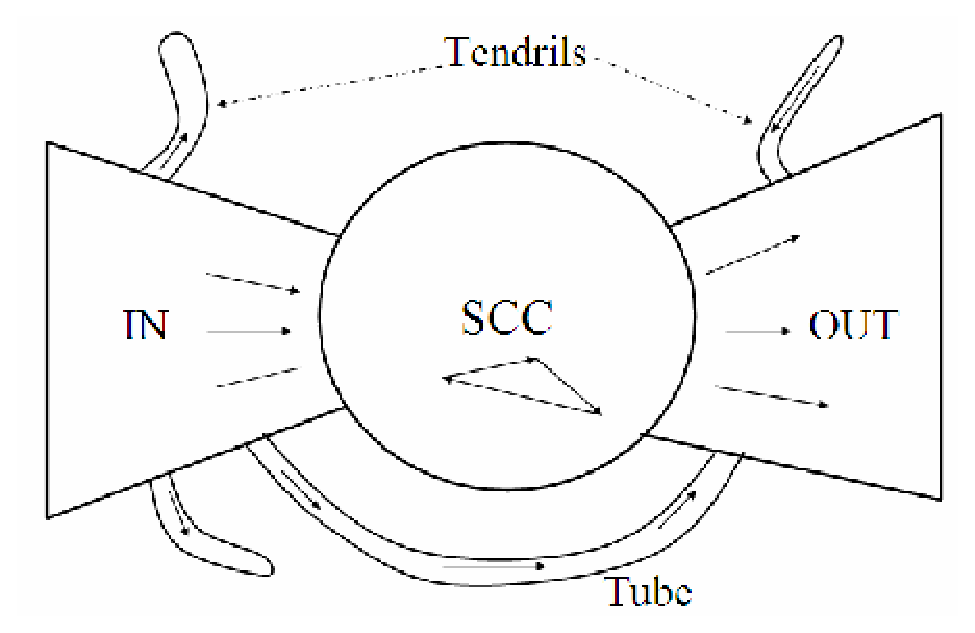
\includegraphics[height=0.8\textheight]{../pics/web-bowtie-bw.eps}  
\end{center}
\blu{SCC}: Strongly Connected Core --- can travel from any page to any page


\myslide{Anchor Text}

\begin{itemize}
\item Recall how hyperlinks are written: \vspace{-1ex}
\begin{verbatim}
<a href="http://path.to.there/page/HG803/">HG803: 
Language, Technology and the Internet.</a>
\end{verbatim}
\begin{verbatim}
For more information about Language, Technology and the
Internet, see the <a href="http://..">HG803 Course Page.</a>
\end{verbatim}
\item Link analysis builds on two intuitions:
  \begin{enumerate}
  \item The hyperlink from A to B represents an endorsement of page B, by the creator of page A.

  \item The (extended) anchor text pointing to page B is a good description of page B.
  \end{enumerate}
  \small {This is not always the case; for instance, most corporate websites have a pointer from every page to a page containing a copyright notice.}
\end{itemize}

\myslide{PageRank as Citation analysis}

\begin{itemize}
\item Citation frequency can be used to measure
  the \blu{impact} of an article.
\begin{itemize}
\item Simplest measure: Each article gets one vote -- not
  very accurate.
\end{itemize}
\item On the web: citation frequency = \blu{inlink count}
\begin{itemize}
\item A high inlink count does not necessarily
  mean high quality \ldots
\item \ldots mainly because of link spam.
\end{itemize}
\item Better measure: \blu{weighted} citation frequency or citation rank
\begin{itemize}
\item An article's vote is weighted according to its
  citation impact. 
\item This  can be formalized in a   well-defined way and calculated.
\end{itemize}
\end{itemize}

\myslide{PageRank as Random walk}
\begin{itemize}
\item Imagine a web surfer doing a random walk on the web
\begin{itemize}
\item Start at a random page
\item At each step, go out of the current page along one of
  the links on that page, equiprobably
\end{itemize}
\item In the steady state, each page has a \blu{long-term visit rate}.
  \\ what proportion of the time someone will be there
\item This long-term visit rate is the page's \blu{PageRank}.
\item \blu{PageRank 
=
  long-term visit rate
= steady state robability 
}
\end{itemize}

\myslide{Teleporting -- to get us out of dead ends}
\begin{itemize}
\item At a \blu{dead end}, jump to a random web page with
  probability $1/N$.
\\ ~   \hfill ($N$ is the total number of web pages)
\item At a \blu{non-dead end}, with probability 10\%, jump to a
  random web page (to each with a probability of $0.1/N$).
\item With remaining probability (90\%), go out on a random
  hyperlink.
\begin{itemize}
 \item For example, if the page has 4 outgoing links:
   randomly choose one with probability (1-0.10)/4=0.225
\end{itemize}
\item 10\% is a parameter, the \blu{teleportation rate}.
\item Note: ``jumping'' from a dead end is
independent of teleportation rate.
\end{itemize}

\myslide{Example Graph}
\MyLogo{http://www.ams.org/samplings/feature-column/fcarc-pagerank}
\begin{center}
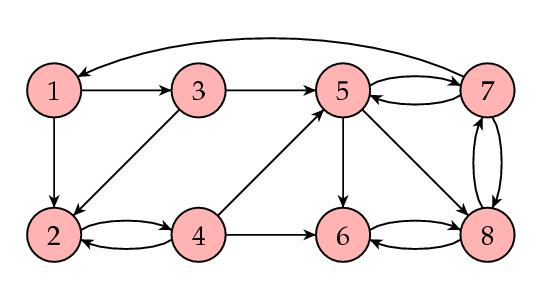
\includegraphics[height=0.8\textheight]{../pics/goodnet.jpg}  
\end{center}
Each inbound link is a positive vote.


\myslide{Example Graph: Weighted}
\begin{center}
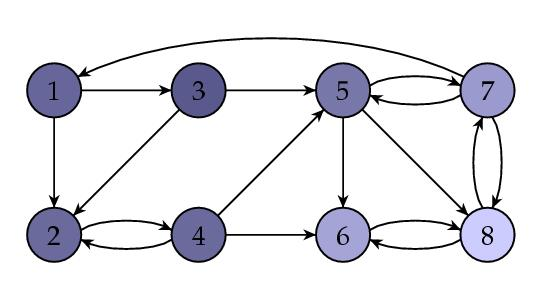
\includegraphics[height=0.8\textheight]{../pics/goodnet-shaded.jpg}  
\end{center}

Pages with higher PageRanks are lighter. 

\myslide{Gaming PageRank}
\MyLogo{}
\begin{itemize}
\item \blu{Link Spam} adding links between pages for reasons other
  than merit.  Link spam takes advantage of link-based ranking
  algorithms, which gives websites higher rankings the more other
  highly ranked websites link to it.  Examples include adding links
  within blogs.
\item \blu{Link Farms} creating tightly-knit communities of pages
  referencing each other, also known humorously as mutual admiration
  societies.
\item \blu{Scraper Sites}  "scrape" search-engine results pages or other sources of content and create "content" for a website. The specific presentation of content on these sites is unique, but is merely an amalgamation of content taken from other sources, often without permission.
\newpage
\item \blu{Comment spam} is a form of link spam in web pages that
  allow dynamic user editing such as wikis, blogs, and guestbooks.
  Agents can be written that automatically randomly select a user
  edited web page, such as a Wikipedia article, and add spamming
  links.
\end{itemize}

\begin{itemize}
\item[!] The \blu{nofollow} link: a value that can be assigned to the rel
attribute of an HTML hyperlink to instruct some search engines that a
hyperlink should not influence the link target's ranking in the search
  engine's index.
  \begin{itemize}
  \item Google does not index the target of a link marked \textbf{nofollow}.
  \item Yahoo! does not include the link in its ranking
  \item \ldots
  \end{itemize}
\end{itemize}

\myslide{Current Status}

\begin{itemize}
\item There is a continuous battle between 
  \begin{itemize}
  \item Search companies, who want to get the most useful page to the user
  \item Page writers, who want to get their page read
  \end{itemize}
\item \emp{All metrics get gamed}
\end{itemize}

\myslide{Digital object identifier}
\begin{itemize}
  \item \blu{DOI}: a string used to uniquely identify an electronic document or object
  \begin{itemize}
  \item Metadata  about the object is stored with the DOI name
  \item The metadata includes a location, such as a URL
  \item The DOI for a document is permanent,  the metadata may change
  \item Gives a Persistent Identifier (like ISBN)
  \end{itemize}
\item  The DOI system is implemented through a federation of registration agencies coordinated by the International DOI Foundation
\item By late 2009 approximately 43 million DOI names had been assigned by some 4,000 organizations
\begin{itemize}
\item DOI: \emp{10.1007/s10579-008-9062-z} 
\\ \url{http://www.springerlink.com/content/v7q114033401th5u/}
\end{itemize}
\end{itemize}





\section{Conclusions}

\myslide{Revolutions in Language Technology}
\begin{itemize}
  \item Speech (Language itself)
  \item Writing (invented 3-5 times)
  \item Printing  (made writing common)
  \item Digital Text (made writing transferable) 
  \item Hyperlinking (taking writing beyond language) 
  \end{itemize}

\myslide{The Internet}

\begin{itemize}
\item The internet is useful as a tool
  \begin{itemize}
  \item Passively for information access
  \item Actively for collaboration
  \end{itemize}
\item The internet is interesting in and of itself
  \begin{itemize}
  \item As a source of data about existing language
  \item As a source of innovation in language
  \end{itemize}
\end{itemize}


% \myslide{Acknowledgments}

% \begin{itemize}
% \item Many slides from Tim Baldwin's \textit{Web as Data} 
%   \\ (Melbourne University 433-352)
% \item Excellent introduction to Information Retrieval, including web searching:
% \\ Christopher D. Manning, Prabhakar Raghavan and Hinrich Schütze, \textit{Introduction to Information Retrieval}, Cambridge University Press. 2008. 
% \\ \url{http://nlp.stanford.edu/IR-book/information-retrieval-book.html}
% \\ \textit{Determining the vocabulary of terms} deals with tokenization/normalization
% \end{itemize}
%%
%% Future
%%


\myslide{Recommended Texts}
%\bibliographystyle{apalike}
%\ifthenelse{\boolean{cjk}}{\nobibliography{abb,mtg,mtg-cjk,ling}}%
%\nobibliography{abb,mtg,nlp,ling}
\renewcommand{\cite}{\bibentry}

\begin{itemize}\addtolength{\itemsep}{-0.5ex}
\item \blu{\textit{Wikipedia}}
\item \cite{Crystal:2001}
\item \cite{Sproat:2010}
%\item \cite{Bird:Klein:Loper:2009}
\item \cite{Jurafsky:Martin:2008}
\item \cite{Manning:Schuetze:1999}
\item \cite{Manning:Raghavan:Schuetze:2008}
%\item \cite{Hughes:Baldwin:Bird:Nicholson:MacKinlay:2006}
\end{itemize}

\myslide{Complementary Courses}

\begin{itemize}
\item \txx{HG2051 Language and the Computer} --- solving NLP problems with Python: introduces both programming and linguistics
\item  \txx{HG3051 Corpus Linguistics} --- (Pre Req-HG251 waived) This course is an introduction to the fast growing field of corpus linguistics.
\end{itemize}

\end{document}


%%% Local Variables: 
%%% coding: utf-8
%%% mode: latex
%%% TeX-PDF-mode: t
%%% TeX-engine: xetex
%%% End: 
